\section{Week 4}
\underline{\Large \textbf{Free Convection}}


\begin{itemize}
    \item \color{blue} Quiescent fluid \color{black} means motionless fluid.
    \item \color{red}Grashof Number\color{black}
    \begin{align*}
        \text{Gr}_{L} &= \frac{g \beta (T_s- T_{\infty}) L_c^3}{v^2} \\ 
        &= \frac{\text{buoyancy force}}{\text{viscous force}} \\
        \text{where } g &= 9.8, \; \text{m/s}^2 \\
        \beta &= \text{coefficient of volume expansion, }\; k^{-1} \\
        T_s &= \text{surface temp.},\;C^{\circ} \\
        T_{\infty} &= \text{fuild temp. far away from surface,}\; C^{\circ}\\
        L_c &= \text{characteristic length, m}\\
        v &= \text{kinematic viscosity of fluid, }\;m^2/s
    \end{align*}
    Note that $\beta = 1/T_f$ for ideal gases.
    \item \color{red} Rayleigh Number\color{black}
    \begin{align*}
        \text{Ra}_L &= \text{Gr}_L \text{Pr}\\
        &= \frac{g\beta (T_s - T_{\infty})L_c^3}{v \alpha } \\
        \text{where } \alpha &= \text{thermal diffusivity} \\
    \end{align*}
    Note that $L_c = $ length parallel to gravity for vertical plates, and $L_c=A_s / P$ for horizontal plates. 
\end{itemize}
\underline{\textbf{Mixed Convection}}
\begin{itemize}
    \item Effects of \color{blue} forced \color{black} and \color{blue} free convection \color{black} are
    \begin{itemize}
        \item comparable if $\text{Gr}_L/\text{Re}_L^2 \approx 1$
        \item free convection dominates if $\text{Gr}_L/\text{Re}_L^2 >> 1$
        \item forced convection dominates if $\text{Gr}_L/\text{Re}_L^2 << 1$
    \end{itemize}
\end{itemize}

\textbf{\underline{\color{red}Vertical Plate\color{black}}}
\begin{itemize}
    \item Transition occurs at a critical Rayleigh number of
    \begin{equation*}
        \text{Ra}_{x,c} = \text{Gr}_{x,c}\text{Pr} \approx 10^9
    \end{equation*}
    \item Heat Transfer Correlations for Mixed Convection:
    \begin{align*}
        \text{Nu}^n &\approx \text{Nu}_{FC}^{n} \pm \text{Nu}_{NC}^{n} \\
        \text{where } n &\approx 3 \\
        \text{Nu}_{FC} &= \text{Nusselt number for forced convection} \\
        \text{Nu}_{NC} &= \text{Nusselt number for natural convection}\\
        + &= \text{assisting and transverse flows}\\
        - &= \text{opposing flows}
    \end{align*}
    \item Empirical Heat Transfer Correlations
    \begin{itemize}
        \item Laminar: $10^4<\text{Ra}<10^9$
        \begin{equation*}
            \overline{\text{Nu}} = 0.59 \text{Ra}_L^{1/4}
        \end{equation*}
        \item Turbulent: $10^{10} < \text{Ra} < 10^{13}$
        \begin{equation*}
            \overline{\text{Nu}} = 0.1 \text{Ra}^{1/3}_{L}
        \end{equation*}
        \item All conditions apply
        \begin{equation*}
            \overline{\text{Nu}}_L = \left\{ 0.825+ \frac{0.387\text{Ra}_{L}^{1/6}}{\left[1+(0.492/\text{Pr})^{9/16}\right]^{8/27}} \right\}^2
        \end{equation*} 
    \end{itemize}
\end{itemize}
\textbf{\underline{\color{red}Horizontal Plate\color{black}}}
\begin{itemize}
    \item Nusselt number (applies to \color{blue} hot surface facing upward \color{black} OR \color{blue} cold surface facing downward\color{black})
    \begin{itemize}
        \item Laminar: $10^4<\text{Ra}_L<10^7$
        \begin{equation*}
            \overline{\text{Nu}}_L = 0.54 \text{Ra}_{L}^{1/4}
        \end{equation*}
        \item Turbulent: $10^7<\text{Ra}_L<10^{11}$ and $\forall \text{Pr}$
        \begin{equation*}
            \overline{\text{Nu}}_L = 0.15 \text{Ra}_L^{1/3}
        \end{equation*}
        These correlations can be used for \color{blue} a variety of different plate shapes \color{black} when the characteristic length $L_c$ is defined as $L_c \equiv \frac{A_s}{P}$
    \end{itemize}
    \item Nusselt number (applies to \color{blue} hot surface facing downward \color{black} OR\color{blue} cold surface facing upward\color{black})
    \begin{itemize}
        \item Laminar $10^5 < \text{Ra}_L<10^{10}$ and $\text{Pr}>0.7$
        \begin{equation*}
            \overline{\text{Nu}}_L = 0.27 \text{Ra}_L^{1/4}
        \end{equation*}
    \end{itemize}
    Plate acts as an obstruction. 
\end{itemize}
\textbf{\underline{\color{red}Horizontal Hot Cylinder\color{black}}}

Churchill-Chu correlation for free convection:
\begin{align*}
    \overline{\text{Nu}}_D &= \left\{0.60 + \frac{0.387 \text{Ra}_D^{1/6}}{\left[1+(0.559/\text{Pr})^{9/16}\right]^{8/27}}\right\}^2\\
    \text{for }\text{Ra}_D &< 10^{12}
\end{align*}
\textbf{\underline{\color{red}Hot Sphere\color{black}}}
\begin{itemize}
    \item Applicable to all conditions associated with spheres:
    \begin{equation*}
        \overline{\text{Nu}}_D = 2 + \frac{0.589 \text{Ra}_D^{1/4}}{\left[1+(0.469/\text{Pr})^{9/16}\right]^{4/9}}
    \end{equation*}
\end{itemize}


\underline{\Large \textbf{Heat Exchangers}}

\vspace{0.5cm}
\underline{ \textbf{Types of Heat Exchanger}}
\begin{itemize}
    \item Concentric-tube heat exchangers
    \begin{figure}[H]
        \centering
        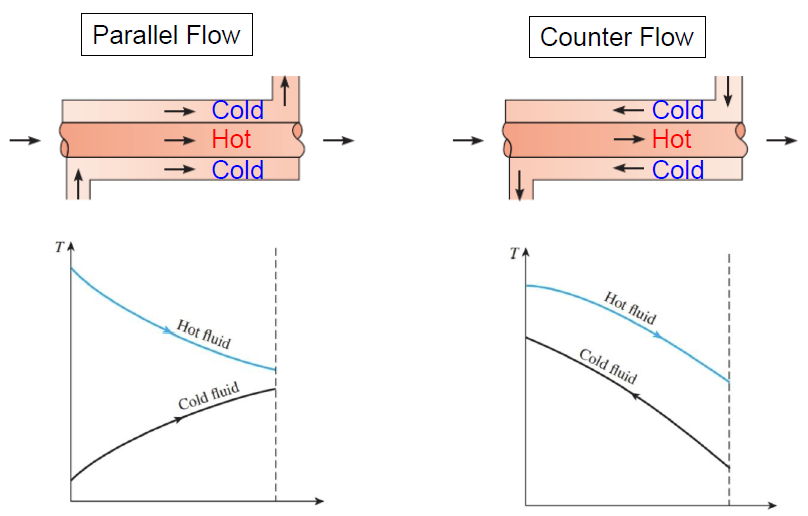
\includegraphics[width=1.0\linewidth]{images/concentric_tube_heat_exchangers.png}
    \end{figure}
    Counter-flow allows the exit temperatures of both fluids to be different.
    \item Cross-flow heat exchangers
    \begin{figure}[H]
        \centering
        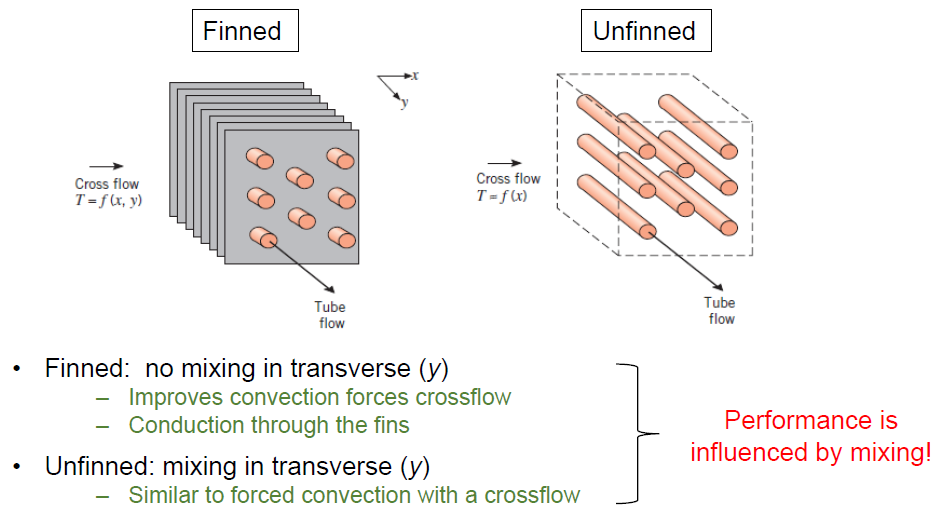
\includegraphics[width=1.0\linewidth]{images/cross_flow_heat_exchanger.png}
    \end{figure}
    \item Shell-and-Tube heat exchanger
    \begin{figure}[H]
        \centering
        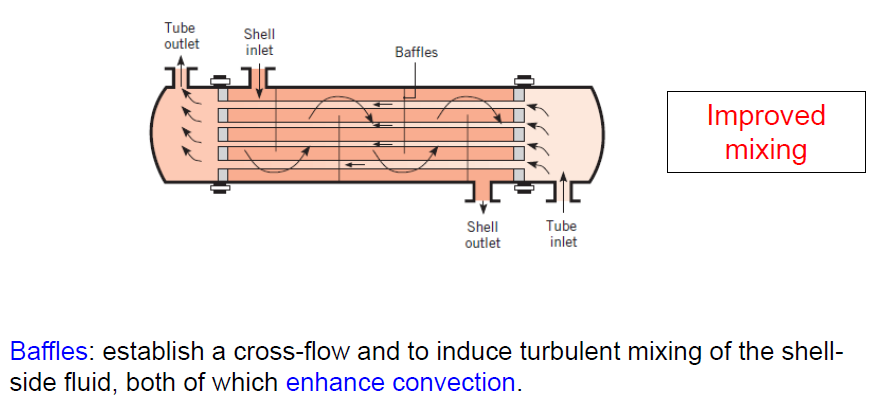
\includegraphics[width=1.0\linewidth]{images/shell_and_tube_heat_exchanger.png}
    \end{figure}
    \item Compact heat exchanger
    \begin{figure}[H]
        \centering
        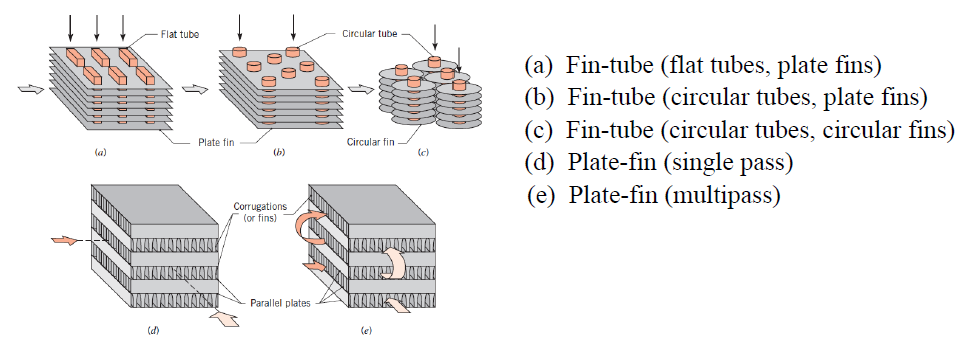
\includegraphics[width=1.0\linewidth]{images/compact_heat_exchanger.png}
    \end{figure}
\end{itemize}
\underline{ \textbf{Overall heat transfer coefficient \color{red}U\color{black}}}
\begin{itemize}
    \item heat gained in cold fluid (c) = heat lost from hot fluid (h)
    \begin{equation*}
        U = \frac{1}{\frac{1}{h_i}+\frac{1}{h_o}}
    \end{equation*}
    \begin{equation*}
        \frac{1}{UA} = \frac{1}{(UA)_c} = \frac{1}{(UA)_h}
    \end{equation*}
    \begin{align*}
        \frac{1}{UA} &= \color{red}\underbrace{\frac{1}{(\eta_O h A)_c} +\frac{1}{(\eta_O h A)_h}}_{\text{Convection}}\color{black} \\
        &+ \color{magenta}\underbrace{\frac{R_{f,c}^{''}}{(\eta_O A)_c} +\frac{R_{f,c}^{''}}{(\eta_O A)_h}}_{\text{Fouling}}\color{black} + \color{blue}\underbrace{R_w }_{\text{Conduction}} \color{black}
    \end{align*}
    \begin{itemize}
        \item $R_{f}^{''}=$ fouling factor for a unit surface area, ($m^2\cdot K/W$)
        \begin{figure}[H]
            \centering
            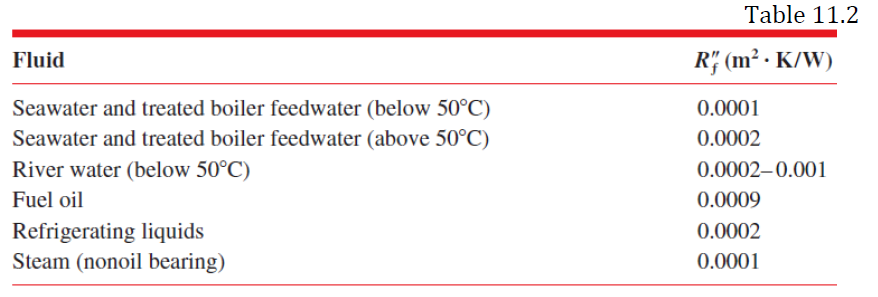
\includegraphics[width=1.0\linewidth]{images/Fouling_table.png}
        \end{figure}
        \item \color{blue} $R_w$ \color{black} = Wall conduction resistance, (K/W) 
        \item $\eta_o = $ Overall surface efficiency of fin array
    \end{itemize}
\end{itemize}
\underline{ \textbf{Methodology for Heat Exchanger Calculations}}
\begin{itemize}
    \item Log Mean Temperature Difference (\color{blue}LMTD\color{black}) Method 
    \begin{align*}
        \dot{Q} &= UA\Delta T_{lm} \\
        \Delta T_{lm} &= \frac{\Delta T_1 - \Delta T_2}{\ln(\Delta T_1 / \Delta T_2)}
    \end{align*}
    \color{red} Evaluation of $\Delta T_1$ and $\Delta T_2$ depends on the heat exchanger types.\color{black}
    \begin{itemize}
        \item Parallel-flow heat exchanger
        \begin{align*}
            \Delta T_1 &= T_{h,i} - T_{c,i} \\
            \Delta T_2 &= T_{h,o} - T_{c,o}
        \end{align*}
        \color{blue} $T_{c,o}$ cannot exceed $T_{h,o}$\color{black}
        \item Counter-flow heat exchanger
        \begin{align*}
            \Delta T_1 &= T_{h,i} - T_{c,o} \\
            \Delta T_2 &= T_{h,o} - T_{c,i}
        \end{align*}
         \color{blue} $T_{c,o}$ can exceed $T_{h,o}$\color{black}
         \item For \color{blue} equivalent values of UA \color{black} and inlet temperatures, \color{blue} $\Delta T_{lm,CF}> \Delta T_{lm,PF}$.
    \end{itemize}
    \item \underline{\textbf{Correction Factor F:}} applies to complex heat exchangers like \color{blue}shell-and-tube \color{black} and \color{blue} cross-flow heat exchangers \color{black}.
    \begin{equation*}
        \Delta T_{lm} = F \Delta T_{lm,CF}
    \end{equation*}
    $F$ measures the \color{red} deviation of $\Delta T_{lm}\;$\color{black} from the corresponding \color{red} counter-flow \color{black} case. 
    \begin{figure}[H]
        \centering
        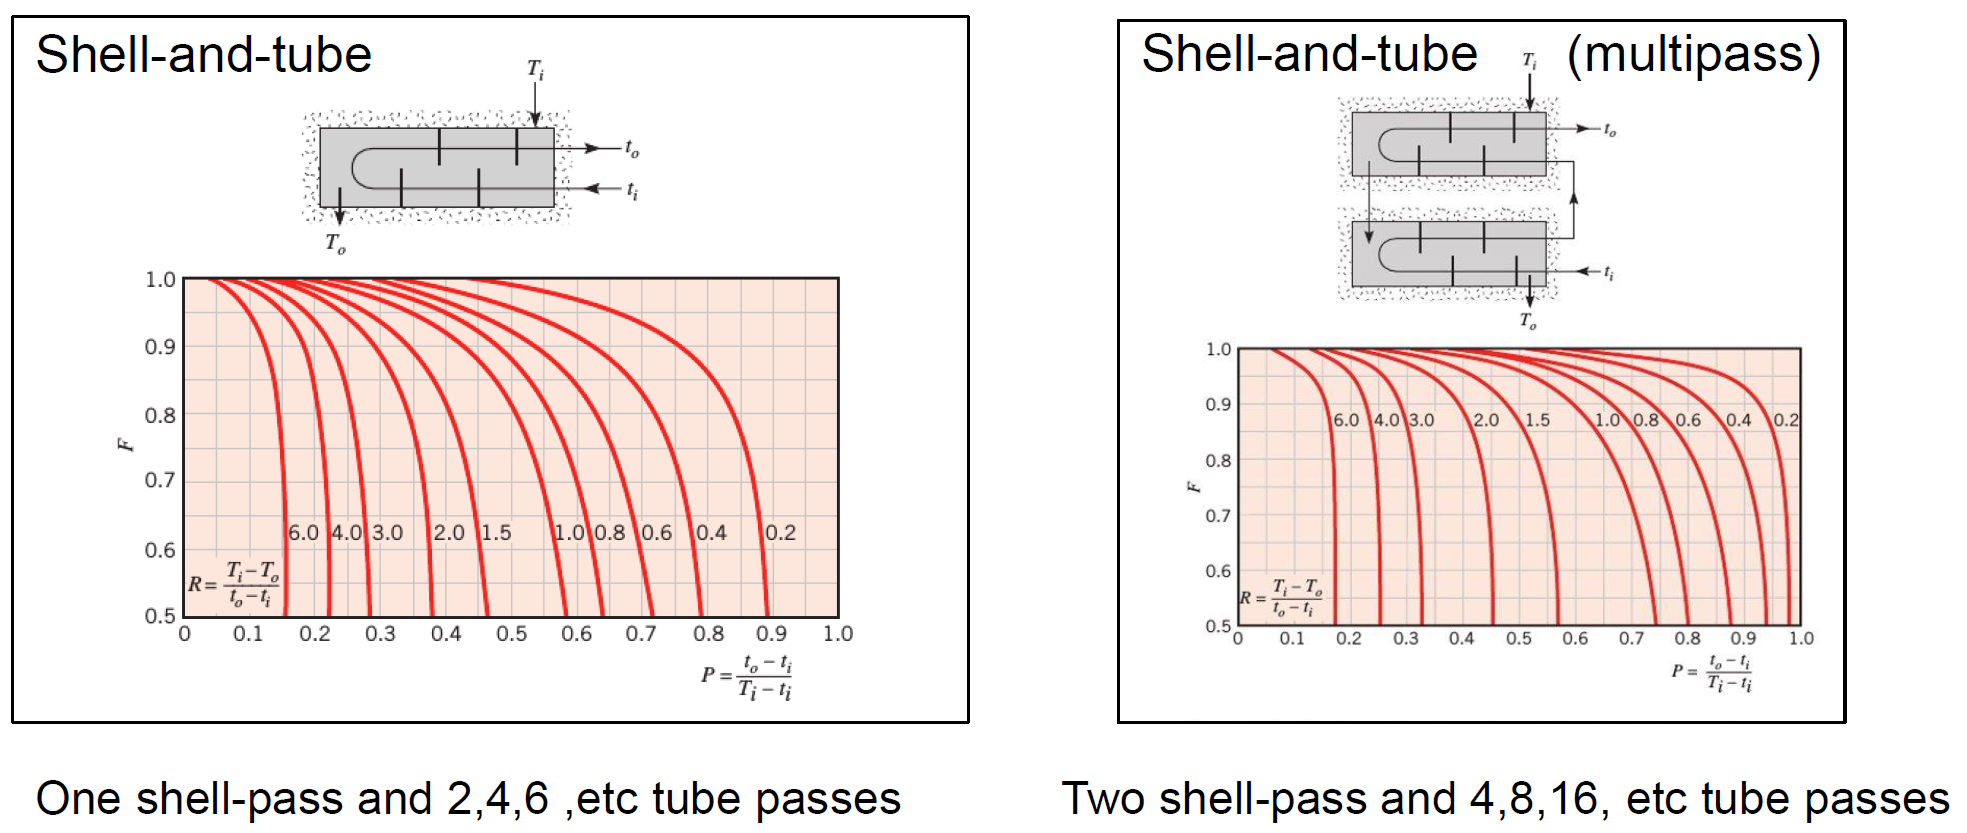
\includegraphics[width=1.0\linewidth]{images/heat_exchanger_correction_factor_1.png}
    \end{figure}
    Note that
    \begin{align*}
        \text{Uppercase} &\rightarrow \text{hot stream} \\
        \text{Lowercase} &\rightarrow \text{cold stream}
    \end{align*}
    \begin{figure}[H]
        \centering
        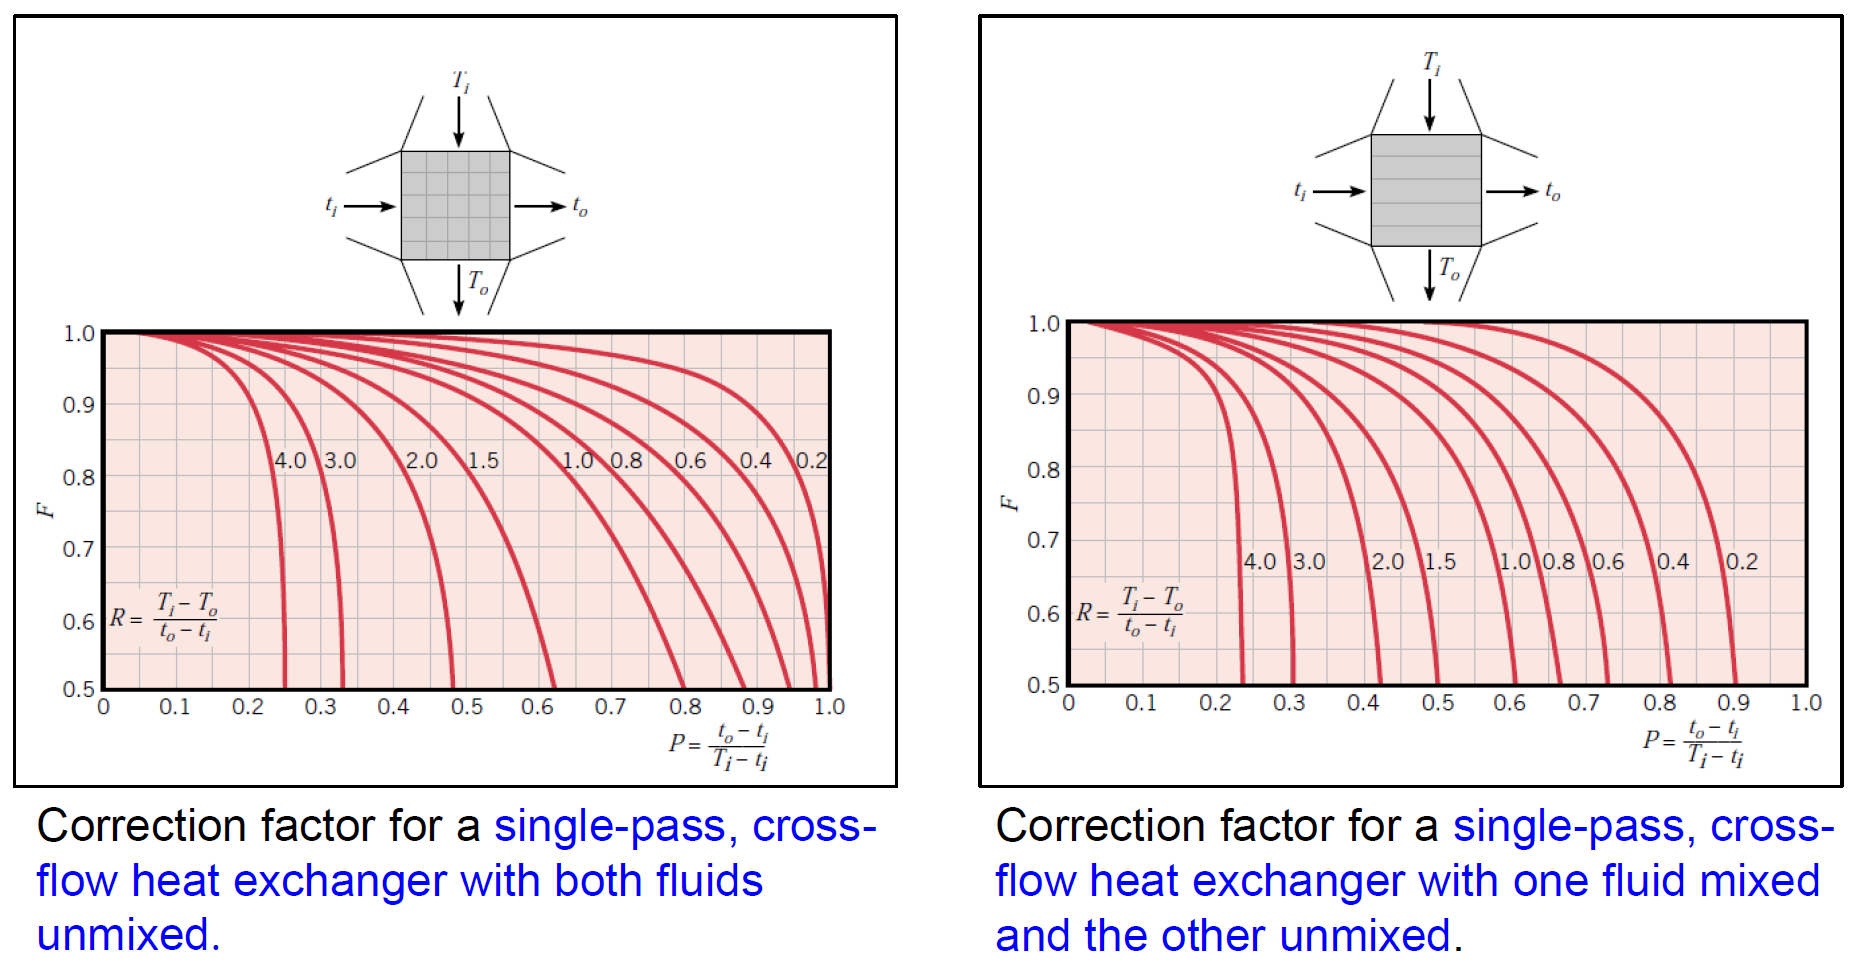
\includegraphics[width=1.0\linewidth]{images/heat_exchanger_correction_factor_2.png}
    \end{figure}
\end{itemize}


\Large \textbf{\underline{Radiation}}


\begin{itemize}
    \item \color{blue} \textbf{Emission:} \color{black} heat transfer from matter resulting in a \color{blue} reduction in its thermal energy. \color{black} 
    \item \color{blue} \textbf{Absorption:} \color{black} radiation may also be intercepted and absorbed by matter, resulting in an increase in thermal energy.
\end{itemize}

\large \textbf{\underline{Emission}}


\begin{itemize}
    \item For gas, liquid, and semitransparent solid, \color{blue} emission \color{black} is a \color{blue} volumetric \color{black} phenomenon.
    \item For opaque solid and liquid, \color{blue} emission \color{black} is a \color{blue} surface phenomenon\color{black} (emission originates from atoms and molecules within 1 $\mu m$ of the surface).
\end{itemize}
\begin{align*}
    \lambda &= \frac{c}{v} \\
    \text{where } \lambda &= \text{wavelength} \\
    v &= \text{frequency} \\
    c &= 2.998\times 10^8 \; m/s
\end{align*}

\large \textbf{\underline{Blackbody Radiation}}
\begin{itemize}
    \item Emissive power at a specific wavelength (Planck distribution)
    \begin{equation*}
        E_{\lambda,b}(\lambda,T) = \frac{C_1}{\lambda^5 [\exp(\frac{C_2}{\lambda T})-1]}
    \end{equation*}
    \begin{itemize}
        \item First radiation constant: $C_1 = 3.742\times 10^8\; W\cdot \mu m^4/m^2$
        \item Second radiation constant: $C_2 = 1.439 \times 10^4\; \mu m \cdot K$
    \end{itemize}
    \item Wien's displacement law:
    \begin{equation*}
        \lambda_{max} T = C_3 = 2898\; \mu m \cdot K
    \end{equation*}
    \item Total emissive power of a blackbody:
    \begin{align*}
        E_b &= \int_{0}^{\infty} E_{\lambda,b} d\lambda = \color{blue}\sigma T^4\color{black} \\
        \text{where } \sigma &= 5.670 \times 10^{-8} W/m^2\cdot K^4
    \end{align*}
    \item Blackbody radiation function $f_{\lambda}$
    \begin{itemize}
        \item $f_{\lambda}$ is a fraction of radiation emitted at $T$ in a fixed wavelength band.
        \item Defined as
        \begin{equation*}
            f_{\lambda}(T) = \frac{\int^{\infty}_{0}E_{\lambda,b}d\lambda }{\sigma T^4}
        \end{equation*}
        \item Use $\lambda\times T$ to find the tabulated value of $f_{\lambda}$
        \begin{figure}[H]
            \centering
            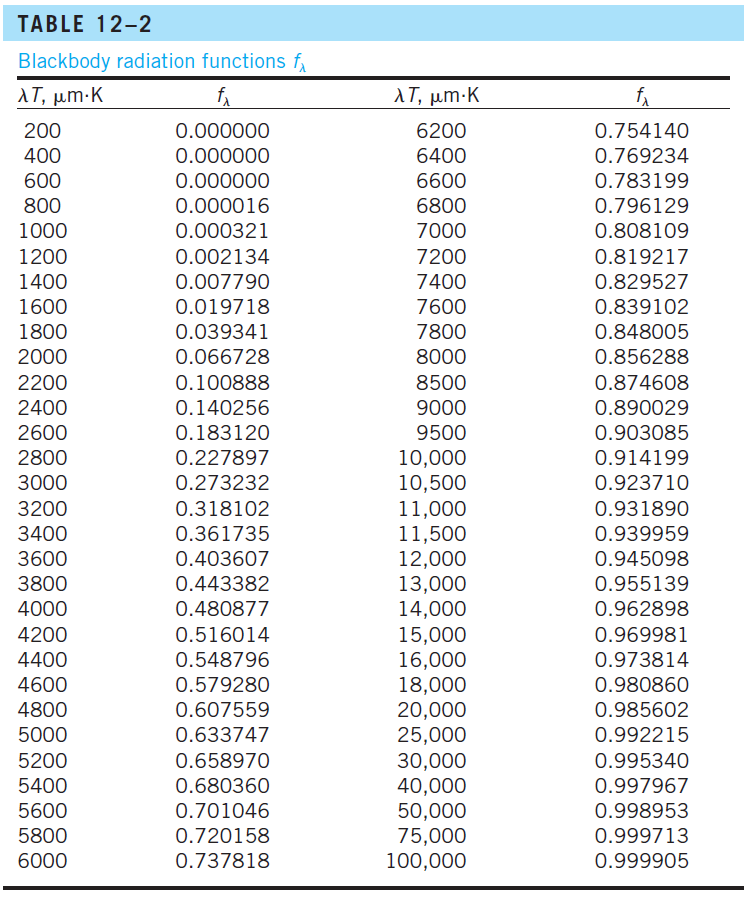
\includegraphics[width=1.0\linewidth]{images/blackbody_radiation_functions.png}
        \end{figure}
    \end{itemize}
\end{itemize}

